% natbib guide (https://gking.harvard.edu/files/natnotes2.pdf)
% \citet     #textual citations, print the abbreviated author list
% \citet*    #textual citations, print the full author list
% \citep     #parenthetical citations, print the abbreviated author list
% \citep*    #parenthetical citations, print the full author list
% \citealt    #the same as \citet but without any parentheses.
% \citealp    #the same as \citep but without any parentheses. 
% \citeauthor{ale91}         #Alex et al.
% \citeauthor*{ale91}        #Alex, Mathew, and Ravi
% \citeyear{ale91}           #1991 
% \citeyearpar{ale91}        #(1991)

\documentclass[english, xcolor=dvipsnames, aspectratio=169]{beamer}

% Text encoding
\usepackage[english]{babel}

% Justify text (package and function)
% \apptocmd{command}{code}{success}{failure}
\usepackage{ragged2e}
\apptocmd{\frame}{}{\justifying}{} 
% Justify text in \item
\newcommand{\itemj}{\item \justifying}

% If...else package
\usepackage{ifthen}

% Package to set transparent background image
\usepackage{tikz}

% Include image package
\usepackage{graphicx}
% Set default path for images
\graphicspath{ {./imgs/} }
% Set figure number when included
\setbeamertemplate{caption}[numbered]

% Bibliography packages
\usepackage[sort, round]{natbib}
\bibliographystyle{plainnat}

% Define colors variables
\definecolor{red}{rgb}{0.631, 0.094, 0.094} % primary color
\definecolor{grey}{rgb}{0.3686, 0.5255, 0.6235} % secondary color

% Set theme palette colors
\setbeamercolor{palette primary}{bg=blue,fg=white}
\setbeamercolor{palette secondary}{bg=blue,fg=white}
\setbeamercolor{palette tertiary}{bg=blue,fg=white}
\setbeamercolor{palette quaternary}{bg=blue,fg=white}
% strucure means itemize, enumerate, etc
\setbeamercolor{structure}{fg=blue} 

% Set bibliography colors
\setbeamercolor{bibliography item}{fg=blue}
\setbeamercolor{bibliography entry author}{fg=black}
\setbeamercolor{bibliography entry title}{fg=black}
\setbeamercolor{bibliography entry location}{fg=black}
\setbeamercolor{bibliography entry note}{fg=black}
% Replaces book icon in bibliography with enumeration
\setbeamertemplate{bibliography item}{[\theenumiv]}

% Table of contents style
% \setbeamertemplate{section in toc}[sections numbered]
% \setbeamertemplate{subsection in toc}[subsections numbered]
\setbeamertemplate{section in toc}[circle]
\setbeamertemplate{subsection in toc}[ball unnumbered]

% Header with navigation bar
\setbeamertemplate{headline}
{
    \leavevmode
    \hbox{
    \begin{beamercolorbox}[wd=\paperwidth,ht=2.5ex,dp=1.125ex]{palette quaternary}
    \insertsectionnavigationhorizontal{\paperwidth}{}{\hskip0pt plus1filll}
    \end{beamercolorbox} 
    }
}
% Footer with custom caption
\setbeamertemplate{footline}
{
    \leavevmode
    \hbox{
    \begin{beamercolorbox}[wd=.33\paperwidth,ht=2.6ex,dp=1ex,center]{palette quaternary}
    \usebeamerfont{author in head/foot}\insertshortauthor\hspace*{1ex}
    \end{beamercolorbox}
    \begin{beamercolorbox}[wd=.33\paperwidth,ht=2.6ex,dp=1ex,center]{palette quaternary}
    \usebeamerfont{institute in head/foot}\insertshortinstitute
    \end{beamercolorbox}
    \begin{beamercolorbox}[wd=.33\paperwidth,ht=2.6ex,dp=1ex,center]{palette quaternary}
    \insertframenumber{} / \inserttotalframenumber
    \end{beamercolorbox}}
    \vskip0pt
}

% Global Background must be put in preamble
\usebackgroundtemplate
{
    \tikz\node[opacity=0.3]{
\includegraphics[height=\paperheight, width=\paperwidth]{background.png}};
}

% One line command to print table of contents - two parameters for modes
\newcommand{\customToC}[2]
{
    \begin{frame}{Overview}
    \tableofcontents[#1,#2]
    \end{frame}
}

% Command to plot centered figure
% Parameters: #1=image name, #2=caption 
\newcommand{\includefigure}[2]
{
    \begin{figure}[h]
    \caption{#2}
    \centering
    \includegraphics[width=0.5\textwidth]{#1}
    \end{figure}
}

% Command to set section name as variable (\renewcommand to update)
\newcommand{\sectiontitle}{}
% Command to set subsection name as variable (\renewcommand to update)
\newcommand{\subsectiontitle}{}


% Title page
\title{Digital Communication System on Gaussion Noise using QPSK modulation and LDPC}
%\subtitle{Subtitle}
\author{H. P. Quang, H. L. Dang, H. K. Do}
\institute{University of Science and Technology}
% Date
\day=31\relax
\month=11\relax
\year=2022\relax

\begin{document}

\frame{\titlepage}

% Complete table of contents (ToC)
% \customToC{hideallsubsections}{}
\customToC{}{}

% Section name and highlighted ToC
\renewcommand{\sectiontitle}{Communication Age}
\section{\sectiontitle}
\customToC{currentsection,hideothersubsections}{}

\begin{frame}{\sectiontitle}
    \begin{itemize}
    	\itemj of businesses primarily use email to communicate with
    	their clients, as opposed to online tools (16\%) phone
    	calls (9\%) and face-to-face (5\%). \citet{CommunicationsStatistics2020} 
    \end{itemize}
	\begin{figure}
		\centering
		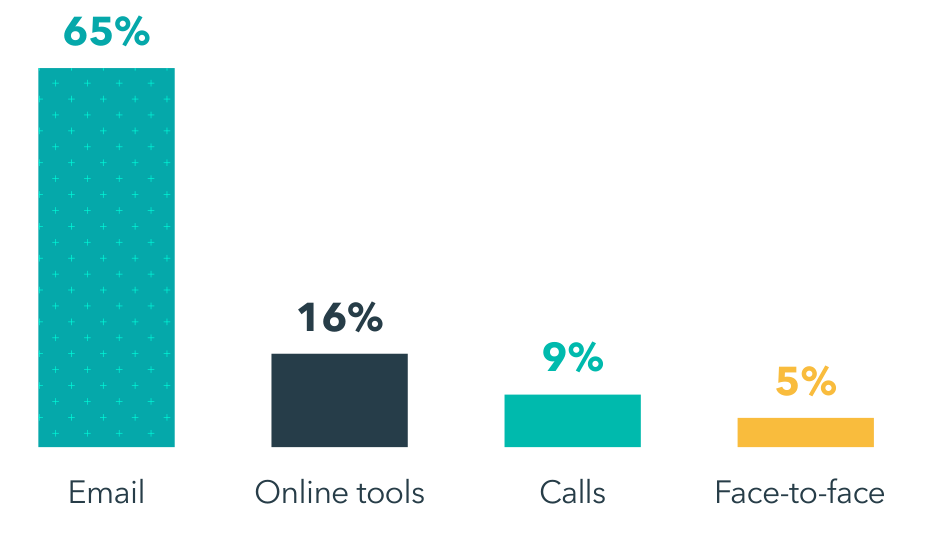
\includegraphics[width=.5\textwidth]{imgs/comway.png}
		\caption{Ways of Communication Statistics}
		\label{fig:com2020}
	\end{figure}
\end{frame}

% Section name and highlighted ToC
\renewcommand{\subsectiontitle}{SOTA Solution}
\subsection{\subsectiontitle}
\begin{frame}{\subsectiontitle}
    \begin{itemize}
        \item Analog modulation methods:
        \begin{itemize}
        	\item Amplitude Modulation (AM): DSB, SSB, VSB, etc
        	\item Angle Modulation (AM): FM, PM, etc
        \end{itemize} 
        \item Digital modulation methods:
        \begin{itemize}
        	\item Phase-shift keying: PSK
        	\item Frequency-shift keying: FSK
        	\item Amplitude-shift keying: ASK
        	\item Quadrature amplitude modulation: QAM
        \end{itemize} 
    \end{itemize}
    
\end{frame}

% Section name and highlighted ToC
\renewcommand{\sectiontitle}{Methodology}
\section{\sectiontitle}
\customToC{currentsection,hideothersubsections}{}

\begin{frame}{\sectiontitle}
    Construct a simulated communication system working on white noise environment using:
    \begin{itemize}
    	\item Quadrature Phase Shift Keying (QSPK) modulation
    	\item Low Density Parity Check (LDPC) code
    	\item BER 
    \end{itemize}
\end{frame}

% Section name and highlighted ToC
\renewcommand{\subsectiontitle}{QPSK}
\subsection{\subsectiontitle}
%\customToC{currentsection,hideothersubsections}{}

\begin{frame}{\subsectiontitle}
    
\end{frame}

\renewcommand{\subsectiontitle}{LDPC}
\subsection{\subsectiontitle}
%\customToC{currentsection,hideothersubsections}{}

\begin{frame}{\subsectiontitle}
	
\end{frame}

\renewcommand{\subsectiontitle}{White Noise}
\subsection{\subsectiontitle}
%\customToC{currentsection,hideothersubsections}{}

\begin{frame}{\subsectiontitle}
	
\end{frame}

\renewcommand{\sectiontitle}{Experiement}
\section{\sectiontitle}
\customToC{currentsection,hideothersubsections}{}

% Section name and highlighted ToC
\renewcommand{\subsectiontitle}{Experimental Setup}
\subsection{\subsectiontitle}

\begin{frame}{\subsectiontitle}

\end{frame}

% Section name and highlighted ToC
\renewcommand{\subsectiontitle}{Experimental Result}
\subsection{\subsectiontitle}
% \customToC{currentsection,hideothersubsections}{}

% Slide with four figures
\begin{frame}{\subsectiontitle}
	
\end{frame}

% Import bibliography from file sample.bib
\begin{frame}[t, allowframebreaks]
\frametitle{References}
\bibliography{sample}
\end{frame}

\end{document}